\section{Apresentação}

\begin{frame} % Capa
    \titlepage
\end{frame}

\begin{frame}[c]{Apresentação}
    \begin{itemize}
        \item Professor Rodrigo de Farias Gomes
        \item Telefone (somente mensagens): (92) 9 9405-1724
        \item E-mail: shpnft@gmail.com
    \end{itemize}
\end{frame}

\begin{frame}{Ementa de Geometria Analítica}
    \begin{itemize}
        \item Vetores no plano e no espaço
        \item Operações com vetores: adição, multiplicação por escalar e produto interno
        \item Produto interno, produto vetorial e produto misto
        \item Equação vetorial de uma reta
        \item Equação do plano
        \item Distância entre ponto e plano, entre reta e plano e entre planos
        \item Interpretação geométrica de sistemas de equações lineares com duas incógnitas
        \item Sistemas equações lineares e seu significado geométrico
        \item Equações reduzidas da elipse, hipérbole e parábola
        \item Quádricas
    \end{itemize}
\end{frame}

\begin{frame}{Avaliação}
    \begin{itemize}
        \item A avaliação será na forma de 3 notas: \(N_1\), \(N_2\) e \(N_3\)
        \item A média dos exercícios escolares (\(MEE\)) será dada por
            \[
                MEE=\frac{N_1+N_2+N_3}{3}
            \]
        \item Se \(MEE \geq 8,0\), então a média final (\(MF\)) será igual à \(MEE\)
        \item Se \(MEE < 8,0\), então
            \[
                MF=\frac{2\times MEE+PF}{3}
            \]
            onde PF é a nota da \textbf{prova final}
        \item Se \(MF \geq 5,0\) e a frequência em sala for maior que 75\%, o aluno está aprovado
    \end{itemize}
\end{frame}

\begin{frame}{Livro Texto}
    \begin{center}
        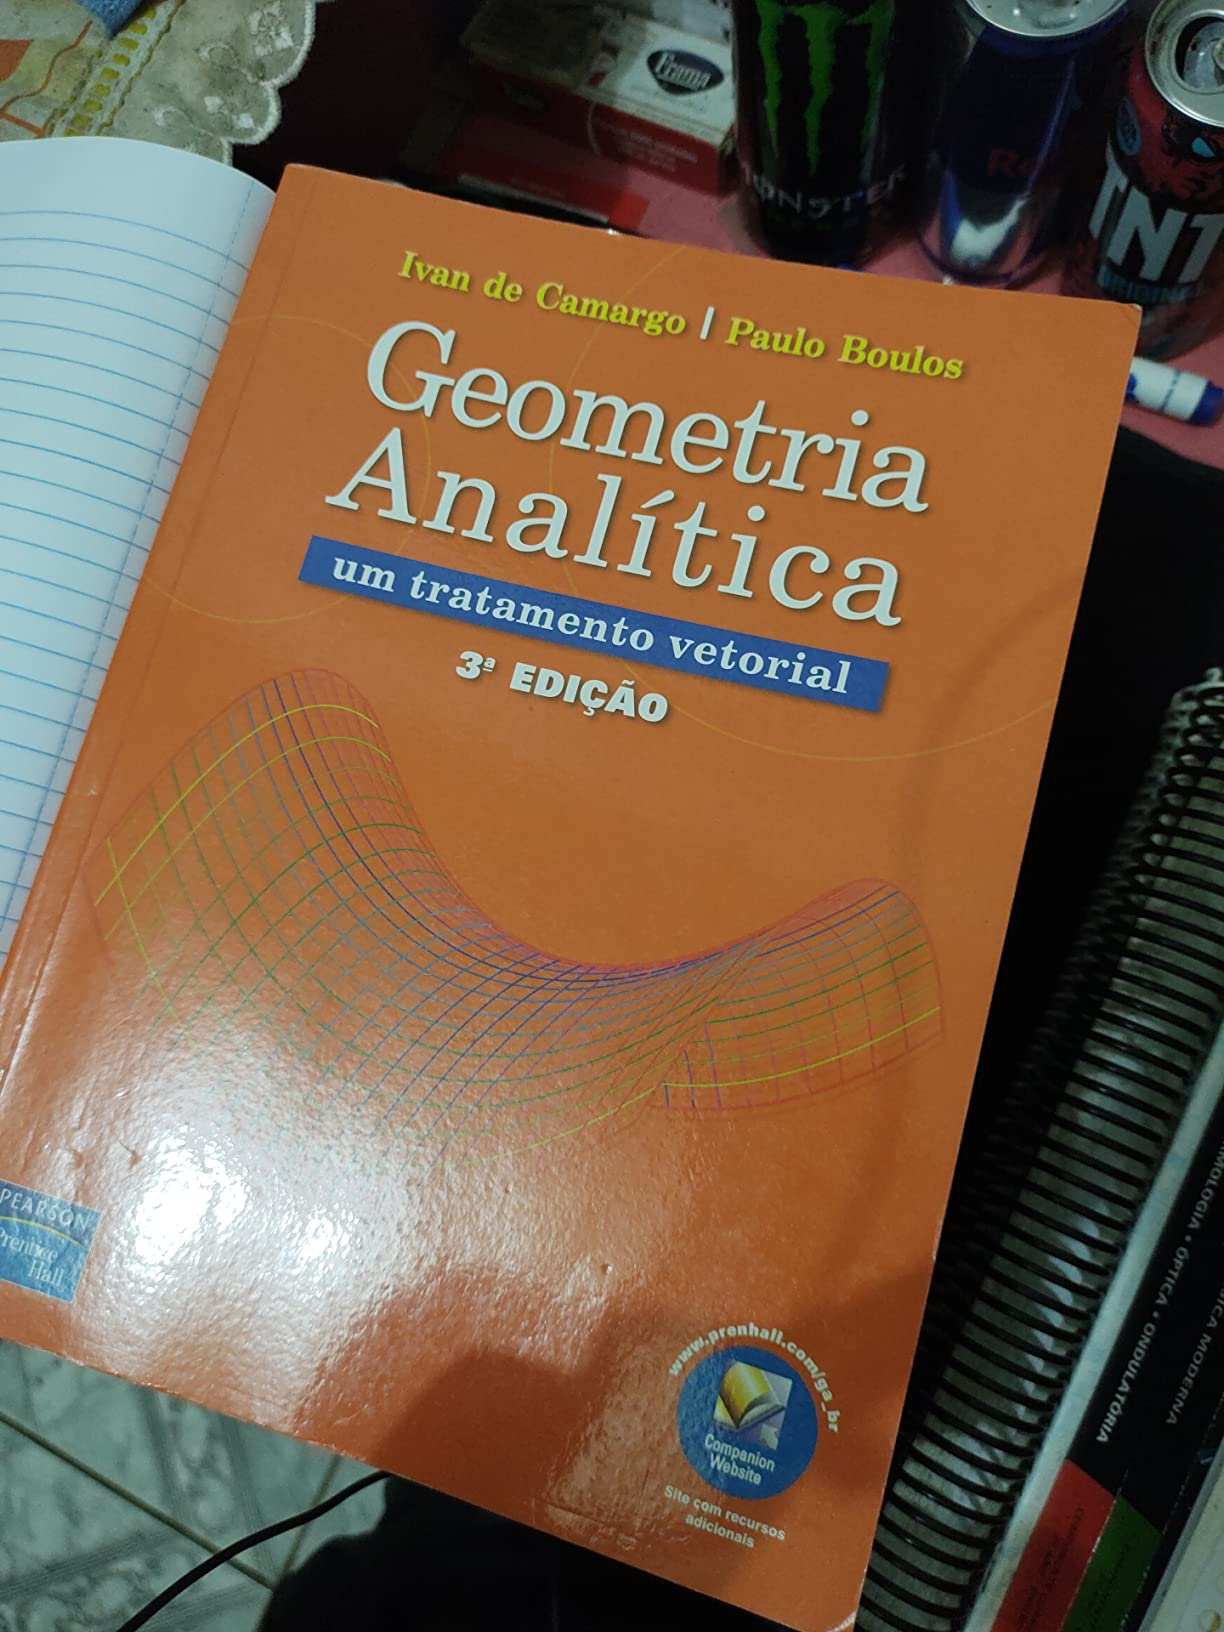
\includegraphics[height=0.8\textheight]{images/livro-texto}
    \end{center}
\end{frame}

\begin{frame}{Geometria plana}
    \begin{itemize}
        \item Ponto
        \item Reta
            \begin{itemize}
                \item Segmento de reta
            \end{itemize}
        \item Plano
        \item Polígonos
            \begin{itemize}
                \item Triângulos
                \item Quadriláteros (quadrado, paralelogramo, losango)
                \item Pentágonos, hexágonos etc
                \item<2> Perímetro e área
            \end{itemize}
        \item Círculo
            \begin{itemize}
                \item Circunferência
                \item Cordas
                \item Arcos
                \item<2> Raio, diâmetro, comprimento e área
            \end{itemize}
    \end{itemize}
\end{frame}

\section{Vetores}

\begin{frame}{Nomenclatura e notação}
    \begin{itemize}[<+->]
        \item Dois pontos distintos \(A\) e \(B\) do espaço determinam uma reta \(r\)
        \item O segmento de reta entre \(A\) e \(B\) é a parte da reta compreendida entre esses dois pontos
        \item O \textbf{segmento orientado} com origem \(A\) e extremidade \(B\) será indicado por \((A,B)\)
        \item Vamos considerar os pontos como segmentos orientados sem ''tamanho'' (nulos)
        \item Ou seja, o ponto \(A\) pode ser identificado como o segmento orientado \((A,A)\)
        \item O segmento orientado \((A,B)\) é \textbf{equipolente} ao segmento orientado \((A',B')\) se:
            \begin{itemize}[<.->]
                \item forem ambos nulos ou
                \item tiverem a mesma direção, mesmo comprimento e mesmo sentido
            \end{itemize}
        \item Indica-se a equipolência entre \((A,B)\) e \((A',B')\) por
            \[
                (A,B) \sim (A',B')
            \]
    \end{itemize}
\end{frame}

\begin{frame}{Vetores}
    \begin{itemize}
        \item<+-> O \textbf{vetor} determinado por um segmento orientado \((A,B)\) é o conjunto de todos os segmentos orientados
            do espaço que são \textbf{equipolentes} ao segmento orientado \((A,B)\)
        \item<.-> O vetor determinado por \((A,B)\) pode ser indicado por \(\vec{AB}\) ou por uma letra minúscula quando não se
            quer destacar um representante (por exemplo, \(\vec{a}\))
        \item<+-> Note que \((A,B)\) não é a mesma coisa de \(\vec{AB}\): um vetor pode ser representado por uma infinidade
            de segmentos orientados distintos
        \item<.-> Se \((A,B) \sim (A',B')\), então \(\vec{AB} = \vec{A'B'}\) mesmo que \((A,B) \neq (A',B')\)
        \item<+-> \textbf{Vetor nulo} é um vetor que tem como representante um  segmento orientado nulo e
            é representado por \(\vec{0}\)
        \item<.-> Se \((A,B)\) representa \(\vec{a}\), o \textbf{vetor oposto} \(-\vec{a}\) pode ser representado pelo
            segmento orientado \((B,A)\)
        \item<+-> \textbf{Norma} ou \textbf{módulo} de um vetor \(\vec{u}\), \(||\vec{u}||\), é o comprimento de qualquer um dos
            seus representantes. Um vetor é \textbf{unitário} se sua norma é 1
    \end{itemize}
\end{frame}

\begin{frame}{Soma de vetores}
    Dados \(\vec{u}\) e \(\vec{v}\), sejam \((A,B)\) um representante qualquer de \(\vec{u}\) e \((B,C)\) o representante
    de \(\vec{v}\). O vetor soma de \(\vec{u}\) com \(\vec{v}\), indicado por \(\vec{u}+\vec{v}\), é o vetor que tem \((A,C)\)
    por representante:
    \[
        \vec{u}+\vec{v}=\vec{AC}
    \]
    \begin{center}
        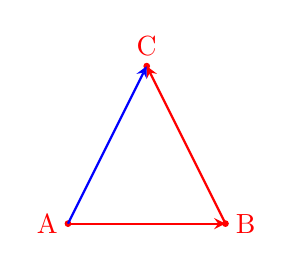
\begin{tikzpicture}[scale=1]
            \draw [red,thick,-stealth] (0,0) node[left] {A} -- (2,0) node [right] {B};
            \draw [fill, red] (0,0) circle (1 pt);
            \draw [fill, red] (2,0) circle (1 pt);
            \draw [fill, red] (1,2) circle (1 pt);
            \draw [red, thick, -stealth] (2,0) -- (1,2) node[above] {C};
            \onslide<2->{
                \draw [blue, thick, -stealth] (0,0) -- (1,2);
            }
        \end{tikzpicture}
    \end{center}

    \onslide<2-> {
        \begin{itemize}
            \item Se os representantes dos vetores a serem somados não forem consecutivos, basta encontrar
                outros representantes
            \item Para determinar o vetor \(\vec{x}=\vec{u}+\vec{v}+\vec{w}+\ldots\), tomam-se representantes consecutivos
                (a origem de cada um coincidindo com a extremidade do anterior) e ''fecha-se o polígono''
        \end{itemize}
    }
\end{frame}

\begin{frame}{Soma de vetores}

    Sejam \(\vec{u}\), \(\vec{v}\) e \(\vec{w}\) vetores quaisquer. Valem as propriedades básicas:

    \begin{enumerate}
        \item \textbf{Propriedade associativa}:
            \((\vec{u}+\vec{v})+\vec{w}=\vec{u}+(\vec{v}+\vec{w})\)
        \item \textbf{Propriedade comutativa}: \(\vec{u}+\vec{v}=\vec{v}+\vec{u}\)
        \item \textbf{Elemento neutro}: \(\vec{u}+\vec{0}=\vec{u}\)
        \item \textbf{Elemento oposto}: \(\vec{u}+(-\vec{u})=\vec{0}\)
    \end{enumerate}
    \pause
    A partir dessas propriedades básicas, podemos obter diversas propriedades derivadas, como por exemplo:
    \begin{itemize}
        \item \(\vec{x}+\vec{u}=\vec{y}+\vec{u} \textcolor{red}{\Rightarrow} \vec{x}=\vec{y}\)
        \item \(\vec{x}+\vec{u}=\vec{u} \textcolor{red}{\Rightarrow} \vec{x}=\vec{0}\)
        \item \(\vec{x}+\vec{u}=\vec{0} \textcolor{red}{\Rightarrow} \vec{x}=-\vec{u}\)
        \item \(\vec{x}+\vec{a}=\vec{b} \textcolor{red}{\Rightarrow} \vec{x}=\vec{b}-\vec{a}\)
        \item \(\vec{u}=\vec{v} \textcolor{red}{\Rightarrow} \vec{u}-\vec{v}=\vec{0}\)
    \end{itemize}
\end{frame}

\begin{frame}{Exemplo 1}
\begin{columns}

\begin{column}[t]{0.38\textwidth}

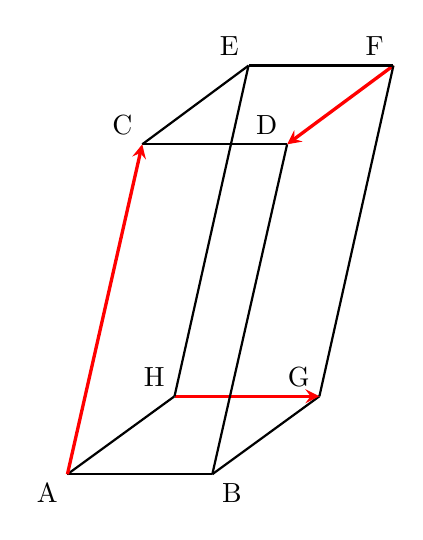
\begin{tikzpicture}[>=stealth]
    \coordinate (A) at (0.35,0.56);
    \coordinate (B) at (2.19,0.56);
    \coordinate (C) at (1.3,4.75);
    \coordinate (D) at (3.14,4.75);
    \coordinate (E) at (2.65,5.75);
    \coordinate (F) at (4.49,5.75);
    \coordinate (G) at (3.55,1.55);
    \coordinate (H) at (1.71,1.55);
    \draw [thick] (A) -- (B);
    \draw [thick] (B) -- (G);
    \draw [very thick, ->, red] (H) -- (G);
    \draw [thick] (H) -- (A);
    \draw [thick] (C) -- (D);
    \draw [very thick, ->, red] (F) -- (D);
    \draw [thick] (F) -- (E);
    \draw [thick] (E) -- (C);
    \draw [very thick,->, red] (A) -- (C);
    \draw [thick] (D) -- (B);
    \draw [thick] (H) -- (E);
    \draw [thick] (F) -- (G);
    \node [below left]  at (A) {A};
    \node [below right] at (B) {B};
    \node [above left]  at (C) {C};
    \node [above left]  at (D) {D};
    \node [above left]  at (E) {E};
    \node [above left]  at (F) {F};
    \node [above left]  at (G) {G};
    \node [above left]  at (H) {H};
\end{tikzpicture}
\end{column}

\begin{column}[t]{0.62\textwidth}
\begin{itemize}
    \item Sejam os vetores \(\vec{AC}\), \(\vec{HG}\) e \(\vec{FD}\)
    \item Vamos calcular \(\vec{AC}+\vec{HG}+\vec{FD}\)
    \item Temos que \(\vec{HG}=\vec{EF}\) (mesma direção, tamanho e sentido)
    \item Temos que \(\vec{AC}=\vec{HE}\) (mesma direção, tamanho e sentido)
\end{itemize}
\end{column}
\end{columns}

\end{frame}

\begin{frame}{Exemplo 1}
\begin{columns}

\begin{column}[t]{0.38\textwidth}

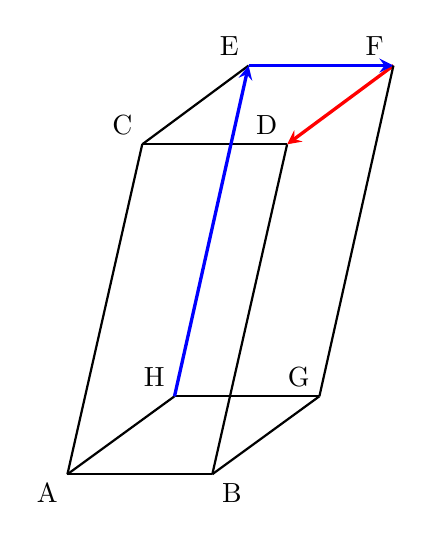
\begin{tikzpicture}[>=stealth]
    \coordinate (A) at (0.35,0.56);
    \coordinate (B) at (2.19,0.56);
    \coordinate (C) at (1.3,4.75);
    \coordinate (D) at (3.14,4.75);
    \coordinate (E) at (2.65,5.75);
    \coordinate (F) at (4.49,5.75);
    \coordinate (G) at (3.55,1.55);
    \coordinate (H) at (1.71,1.55);
    \draw [thick] (A) -- (B);
    \draw [thick] (B) -- (G);
    \draw [thick] (H) -- (G);
    \draw [thick] (H) -- (A);
    \draw [thick] (C) -- (D);
    \draw [very thick, ->, red] (F) -- (D);
    \draw [very thick, ->, blue] (E) -- (F);
    \draw [thick] (E) -- (C);
    \draw [thick] (A) -- (C);
    \draw [thick] (D) -- (B);
    \draw [very thick, ->, blue] (H) -- (E);
    \draw [thick] (F) -- (G);
    \node [below left]  at (A) {A};
    \node [below right] at (B) {B};
    \node [above left]  at (C) {C};
    \node [above left]  at (D) {D};
    \node [above left]  at (E) {E};
    \node [above left]  at (F) {F};
    \node [above left]  at (G) {G};
    \node [above left]  at (H) {H};
\end{tikzpicture}
\end{column}

\begin{column}[t]{0.62\textwidth}
\begin{itemize}
    \item Sejam os vetores \(\vec{AC}\), \(\vec{HG}\) e \(\vec{FD}\)
     \item Vamos calcular \(\vec{AC}+\vec{HG}+\vec{FD}\)
    \item Temos que \(\vec{HG}=\vec{EF}\) (mesma direção, tamanho e sentido)
    \item Temos que \(\vec{AC}=\vec{HE}\) (mesma direção, tamanho e sentido)
    \item Ou seja, podemos trocar \(\vec{AC}\) por \(\vec{HE}\) e \(\vec{HG}\) por \(\vec{EF}\)
    \item \textbf{Ou seja}:
    \[
    \vec{AC}+\vec{HG}+\vec{FD} = \vec{HE}+\vec{EF}+\vec{FD}
    \]
\end{itemize}
\end{column}
\end{columns}

\end{frame}

\begin{frame}{Exemplo 1}
\begin{columns}

\begin{column}[t]{0.38\textwidth}

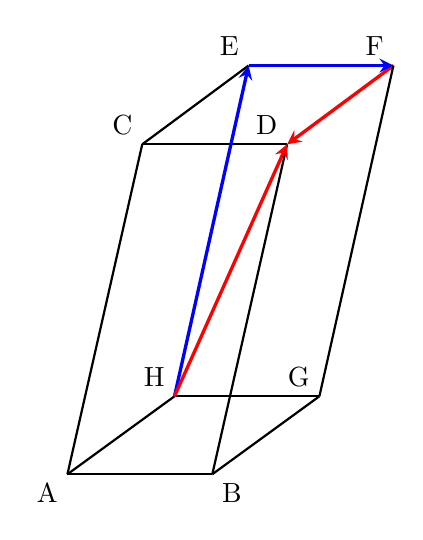
\begin{tikzpicture}[>=stealth]
    \coordinate (A) at (0.35,0.56);
    \coordinate (B) at (2.19,0.56);
    \coordinate (C) at (1.3,4.75);
    \coordinate (D) at (3.14,4.75);
    \coordinate (E) at (2.65,5.75);
    \coordinate (F) at (4.49,5.75);
    \coordinate (G) at (3.55,1.55);
    \coordinate (H) at (1.71,1.55);
    \draw [thick] (A) -- (B);
    \draw [thick] (B) -- (G);
    \draw [thick] (H) -- (G);
    \draw [thick] (H) -- (A);
    \draw [thick] (C) -- (D);
    \draw [very thick, ->, red] (F) -- (D);
    \draw [very thick, ->, blue] (E) -- (F);
    \draw [thick] (E) -- (C);
    \draw [thick] (A) -- (C);
    \draw [thick] (D) -- (B);
    \draw [very thick, ->, blue] (H) -- (E);
    \draw [thick] (F) -- (G);
    \node [below left]  at (A) {A};
    \node [below right] at (B) {B};
    \node [above left]  at (C) {C};
    \node [above left]  at (D) {D};
    \node [above left]  at (E) {E};
    \node [above left]  at (F) {F};
    \node [above left]  at (G) {G};
    \node [above left]  at (H) {H};

    \draw[very thick, ->, red] (H) -- (D);
\end{tikzpicture}
\end{column}

\begin{column}[t]{0.62\textwidth}
\begin{itemize}
    \item Sejam os vetores \(\vec{AC}\), \(\vec{HG}\) e \(\vec{FD}\)
    \item Vamos calcular \(\vec{AC}+\vec{HG}+\vec{FD}\)
    \item Temos que \(\vec{HG}=\vec{EF}\) (mesma direção, tamanho e sentido)
    \item Temos que \(\vec{AC}=\vec{HE}\) (mesma direção, tamanho e sentido)
    \item Ou seja, podemos trocar \(\vec{AC}\) por \(\vec{HE}\) e \(\vec{HG}\) por \(\vec{EF}\)
    \item \textbf{Ou seja}:
    \[
    \vec{AC}+\vec{HG}+\vec{FD} = \vec{HE}+\vec{EF}+\vec{FD}
    \]
    \item Finalmente, temos o vetor \(\vec{HD}\)...
\end{itemize}
\end{column}
\end{columns}

\end{frame}

\begin{frame}{Exemplo 2}
\begin{columns}

\begin{column}[t]{0.38\textwidth}

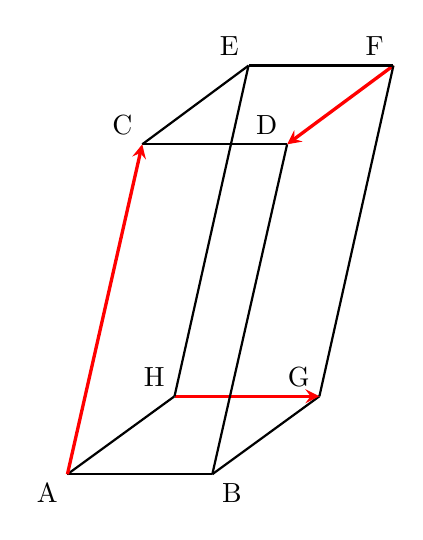
\begin{tikzpicture}[>=stealth]
    \coordinate (A) at (0.35,0.56);
    \coordinate (B) at (2.19,0.56);
    \coordinate (C) at (1.3,4.75);
    \coordinate (D) at (3.14,4.75);
    \coordinate (E) at (2.65,5.75);
    \coordinate (F) at (4.49,5.75);
    \coordinate (G) at (3.55,1.55);
    \coordinate (H) at (1.71,1.55);
    \draw [thick] (A) -- (B);
    \draw [thick] (B) -- (G);
    \draw [very thick, ->, red] (H) -- (G);
    \draw [thick] (H) -- (A);
    \draw [thick] (C) -- (D);
    \draw [very thick, ->, red] (F) -- (D);
    \draw [thick] (F) -- (E);
    \draw [thick] (E) -- (C);
    \draw [very thick,->, red] (A) -- (C);
    \draw [thick] (D) -- (B);
    \draw [thick] (H) -- (E);
    \draw [thick] (F) -- (G);
    \node [below left]  at (A) {A};
    \node [below right] at (B) {B};
    \node [above left]  at (C) {C};
    \node [above left]  at (D) {D};
    \node [above left]  at (E) {E};
    \node [above left]  at (F) {F};
    \node [above left]  at (G) {G};
    \node [above left]  at (H) {H};
\end{tikzpicture}
\end{column}

\begin{column}[t]{0.62\textwidth}
\begin{itemize}
    \item Sejam os vetores \(\vec{AC}\), \(\vec{HG}\) e \(\vec{FD}\)
    \item Vamos calcular \(\vec{AC}-\vec{HG}+\vec{FD}=\vec{AC}+(-\vec{HG})+\vec{FD}\)
    \item Temos que \(-\vec{HG}=\vec{BA}\) (mesma direção, tamanho e sentido oposto ao de \(\vec{HG}\))
    \item Temos que \(\vec{FD}=\vec{GB}\) (mesma direção, tamanho e sentido)
\end{itemize}
\end{column}
\end{columns}

\end{frame}

\begin{frame}{Exemplo 2}
\begin{columns}

\begin{column}[t]{0.38\textwidth}

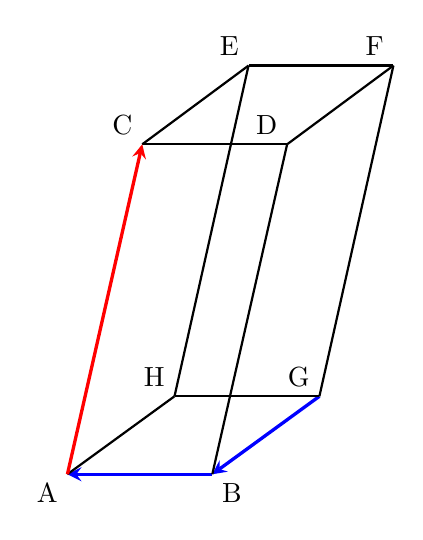
\begin{tikzpicture}[>=stealth]
    \coordinate (A) at (0.35,0.56);
    \coordinate (B) at (2.19,0.56);
    \coordinate (C) at (1.3,4.75);
    \coordinate (D) at (3.14,4.75);
    \coordinate (E) at (2.65,5.75);
    \coordinate (F) at (4.49,5.75);
    \coordinate (G) at (3.55,1.55);
    \coordinate (H) at (1.71,1.55);
    \draw [very thick, <-, blue] (A) -- (B);
    \draw [very thick, <-, blue] (B) -- (G);
    \draw [thick] (H) -- (G);
    \draw [thick] (H) -- (A);
    \draw [thick] (C) -- (D);
    \draw [thick] (F) -- (D);
    \draw [thick] (F) -- (E);
    \draw [thick] (E) -- (C);
    \draw [very thick,->, red] (A) -- (C);
    \draw [thick] (D) -- (B);
    \draw [thick] (H) -- (E);
    \draw [thick] (F) -- (G);
    \node [below left]  at (A) {A};
    \node [below right] at (B) {B};
    \node [above left]  at (C) {C};
    \node [above left]  at (D) {D};
    \node [above left]  at (E) {E};
    \node [above left]  at (F) {F};
    \node [above left]  at (G) {G};
    \node [above left]  at (H) {H};
\end{tikzpicture}
\end{column}

\begin{column}[t]{0.62\textwidth}
\begin{itemize}
    \item Sejam os vetores \(\vec{AC}\), \(\vec{HG}\) e \(\vec{FD}\)
    \item Vamos calcular \(\vec{AC}-\vec{HG}+\vec{FD}=\vec{AC}+(-\vec{HG})+\vec{FD}\)
    \item Temos que \(-\vec{HG}=\vec{BA}\) (mesma direção, tamanho e sentido oposto ao de \(\vec{HG}\))
    \item Temos que \(\vec{FD}=\vec{GB}\) (mesma direção, tamanho e sentido)
    \item Assim:
    \[
    \vec{AC}+(-\vec{HG})+\vec{FD} = \vec{AC}+\vec{BA}+\vec{GB}
    \]
\end{itemize}
\end{column}
\end{columns}

\end{frame}

\begin{frame}{Exemplo 2}
\begin{columns}

\begin{column}[t]{0.38\textwidth}

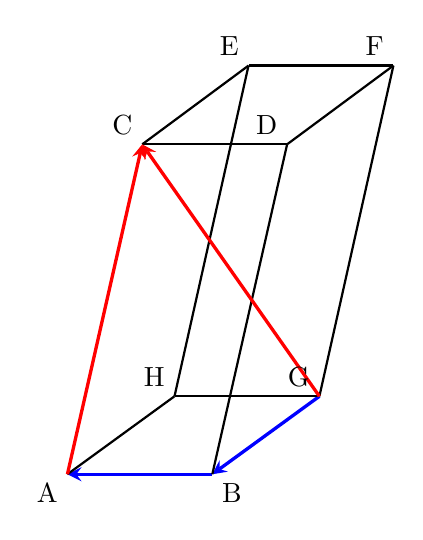
\begin{tikzpicture}[>=stealth]
    \coordinate (A) at (0.35,0.56);
    \coordinate (B) at (2.19,0.56);
    \coordinate (C) at (1.3,4.75);
    \coordinate (D) at (3.14,4.75);
    \coordinate (E) at (2.65,5.75);
    \coordinate (F) at (4.49,5.75);
    \coordinate (G) at (3.55,1.55);
    \coordinate (H) at (1.71,1.55);
    \draw [very thick, <-, blue] (A) -- (B);
    \draw [very thick, <-, blue] (B) -- (G);
    \draw [thick] (H) -- (G);
    \draw [thick] (H) -- (A);
    \draw [thick] (C) -- (D);
    \draw [thick] (F) -- (D);
    \draw [thick] (F) -- (E);
    \draw [thick] (E) -- (C);
    \draw [very thick,->, red] (A) -- (C);
    \draw [thick] (D) -- (B);
    \draw [thick] (H) -- (E);
    \draw [thick] (F) -- (G);
    \draw[very thick,->, red] (G) -- (C);
    \node [below left]  at (A) {A};
    \node [below right] at (B) {B};
    \node [above left]  at (C) {C};
    \node [above left]  at (D) {D};
    \node [above left]  at (E) {E};
    \node [above left]  at (F) {F};
    \node [above left]  at (G) {G};
    \node [above left]  at (H) {H};
\end{tikzpicture}
\end{column}

\begin{column}[t]{0.62\textwidth}
\begin{itemize}
    \item Sejam os vetores \(\vec{AC}\), \(\vec{HG}\) e \(\vec{FD}\)
    \item Vamos calcular \(\vec{AC}-\vec{HG}+\vec{FD}=\vec{AC}+(-\vec{HG})+\vec{FD}\)
    \item Temos que \(-\vec{HG}=\vec{BA}\) (mesma direção, tamanho e sentido oposto ao de \(\vec{HG}\))
    \item Temos que \(\vec{FD}=\vec{GB}\) (mesma direção, tamanho e sentido)
    \item Assim:
    \[
    \vec{AC}+(-\vec{HG})+\vec{FD} = \vec{AC}+\vec{BA}+\vec{GB}
    \]
    \item Finalmente, temos os vetor \(\vec{GC}\)
\end{itemize}
\end{column}

\end{columns}

\end{frame}


%\begin{frame}{Atividade para próxima aula}
%    Resolva o exercício 2-10 do livro texto (página 14), explicando os passos utilizados
%\end{frame}


\begin{frame}{Produto de número real por vetor}
    Sejam \(\alpha\) um número real e \(\vec{v}\) um vetor:

    \begin{enumerate}
        \item Se \(\alpha =0 \) ou \(\vec{v}=\vec{0}\), então \(\alpha \vec{v}=\vec{0}\)
        \item Se \(\alpha \neq 0 \) e \(\vec{v} \neq \vec{0}\), então:
            \begin{enumerate}
                \item \(\alpha\vec{v}\) é paralelo a \(\vec{v}\), que pode ser escrito como
                    \(\alpha\vec{v} // \vec{v}\)
                \item \(\alpha\vec{v}\) e \(\vec{v}\) têm o mesmo sentido se \(\alpha > 0\)
                \item  \(\alpha\vec{v}\) e \(\vec{v}\) têm o sentidos opostos se \(\alpha < 0\)
                \item \(||\alpha\vec{v}||=|\alpha| ||\vec{v}||\) (o módulo do vetor \(\alpha\vec{v}\) é igual ao módulo do número real \(\alpha\) multiplicado pelo módulo do vetor \(\vec{v}\))
            \end{enumerate}
    \end{enumerate}

    \vspace{1cm}

    \textit{Observação}: O módulo de um vetor é o "tamanho" desse vetor e, portanto, não pode ser negativo. Dizer que o módulo de um
    vetor é um número negativo pode causar a destruição do universo conhecido!
\end{frame}

\begin{frame}[c]{Algumas coisinhas...}

    \begin{itemize}
        \item É comum usar o termo \textbf{escalar} para designar um número real em problemas envolvendo vetores (é \textit{chique})
        \item \(\frac{\vec{v}}{\beta}\) ou \(\vec{v}/\beta\) é a mesma coisa que \(\frac{1}{\beta}\vec{v}\)
        \item O vetor unitário \(\frac{\vec{v}}{||\vec{v}||}\) é chamado \textbf{versor} de \(\vec{v}\)
        \item Não se pode usar um vetor como denominador, o seja
            \begin{center}
                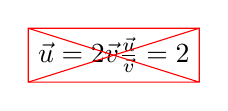
\begin{tikzpicture}
                    \node (equation) {\(\vec{u}=2 \vec{v} \implies \frac{ \vec{u} } { \vec{v} } = 2\) };
                    \onslide<2->{
                        \draw [red] (equation.north west) rectangle (equation.south east) -- (equation.north west);
                        \draw [red] (equation.south west) -- (equation.north east);
                    }
                \end{tikzpicture}
            \end{center}
            \onslide<2->{\textbf{é extremamente errado}}
    \end{itemize}

\end{frame}

\begin{frame}{Propriedades básicas}

    Quaisquer que sejam os escalares \(\alpha\) e \(\beta\) e quaisquer que sejam os vetores \(\vec{u}\), \(\vec{v}\) e \(\vec{w}\),
    valem as igualdades:

    \begin{enumerate}
        \item \(\alpha(\vec{u}+\vec{v})=\alpha\vec{u}+\alpha\vec{v}\)
        \item \((\alpha+\beta)\vec{v}=\alpha\vec{v}+\beta\vec{v}\)
        \item \(1\vec{v}=\vec{v}\)
        \item \(\alpha(\beta\vec{v})=(\alpha\beta)\vec{v}=\beta(\alpha\vec{v})\)
    \end{enumerate}

    \pause
    A partir dessas propriedades básicas, podemos obter diversas propriedades derivadas, como por exemplo:
    \begin{itemize}
        \item \( \vec{v}+\vec{v}=2\vec{v}\)
        \item se \(\alpha \neq 0\), então \(\alpha\vec{v}=\vec{w} \Rightarrow \vec{v}=\vec{w}/\alpha\)
        \item \(\vec{a}=2\vec{b}+\vec{c} \Rightarrow \vec{b}=(\vec{a}-\vec{c})/2\)
        \item \(\alpha\vec{v}=\vec{0} \Rightarrow \alpha = 0 \text{ ou } \vec{v}=\vec{0}\)
        \item se \(\vec{v} \neq \vec{0}\), então \(\alpha\vec{v}=\beta\vec{v} \Rightarrow \alpha=\beta\)
    \end{itemize}
\end{frame}

\begin{frame}{Ninguém perguntou, mas...}
    \begin{tcolorbox}[colback=red!10]
        Propriedades básicas da soma de vetores
        \begin{enumerate}
            \item \textbf{Propriedade associativa}:
                \((\vec{u}+\vec{v})+\vec{w}=\vec{u}+(\vec{v}+\vec{w})\)
            \item \textbf{Propriedade comutativa}: \(\vec{u}+\vec{v}=\vec{v}+\vec{u}\)
            \item \textbf{Elemento neutro}: \(\vec{u}+\vec{0}=\vec{u}\)
            \item \textbf{Elemento oposto}: \(\vec{u}+(-\vec{u})=\vec{0}\)
        \end{enumerate}
    \end{tcolorbox}
    \begin{tcolorbox}[colback=blue!10]
        Propriedades básicas da multiplicação de um vetor por um escalar
        \begin{enumerate}
            \item \(\alpha(\vec{u}+\vec{v})=\alpha\vec{u}+\alpha\vec{v}\)
            \item \((\alpha+\beta)\vec{v}=\alpha\vec{v}+\beta\vec{v}\)
            \item \(1\vec{v}=\vec{v}\)
            \item \(\alpha(\beta\vec{v})=(\alpha\beta)\vec{v}=\beta(\alpha\vec{v})\)
        \end{enumerate}
    \end{tcolorbox}
    Um conjunto com essas propriedades básicas, por exemplo matrizes e polinômios, formam um \textbf{espaço vetorial} que é
    basicamente o assunto mais tratado na disciplina Álgebra Linear
\end{frame}

\begin{frame}{Exercícios}
    \begin{itemize}
        \item[3-10] Resolva, na incógnita \(\vec{x}\), a equação \(2 \vec{x}-3 \vec{u}=10 ( \vec{x} + \vec{v}) \)
        \item[3-11] Resolva os sistemas nas incógnitas \(\vec{x}\) e \(\vec{y}\)
            \begin{columns}
                \begin{column}{0.4\textwidth}
                    \[
                        \text{(a) } \begin{cases}
                            \vec{x}+2 \vec{y}= \vec{u} \\
                            3 \vec{x} - \vec{y} = 2 \vec{u} + \vec{v}
                        \end{cases}
                    \]
                \end{column}

                \begin{column}{0.4\textwidth}
                    \[
                        \text{(b) } \begin{cases}
                            \vec{x} + \vec{y}= \vec{u}- 2\vec{v} \\
                            \vec{x}- \vec{y} = 3 \vec{u}
                        \end{cases}
                    \]
                \end{column}
            \end{columns}

        \item[3-12] Resolva o sistema nas incógnitas \(\vec{x}\), \(\vec{y}\) e \(\vec{z}\)
            \[
                \begin{cases}
                    \vec{x}+ \vec{y} - \vec{z} = \vec{u} + \vec{v} \\
                    \vec{x} - \vec{y} + \vec{z} = \vec{u} - \vec{v} \\
                    -\vec{x} + \vec{y} + \vec{z} = \vec{0}
                \end{cases}
            \]
    \end{itemize}
\end{frame}

% \begin{frame}[fragile]{Vim motion}
%     \centering
%     \begin{tikzpicture}
%         \matrix (m) [matrix of nodes, nodes={align=center, text width=13ex, minimum height=1.4cm, anchor = center,
%         fill=blue!20},
%         every even column/.style = {nodes={fill=red!20}},
%         every even row/.style = {nodes={fill=red!20}},
%         ] {
%             {\textbf{H} \\ start of file} & & & & & \\
%             {\textbf{k} \\ up} & & & & & \\
%             {\textbf{0} \\ start of line} & {\textbf{b} \\ previous word} &
%             {\textbf{h} \\ left} & {\textbf{l} \\ right} & {\textbf{w} \\ next word} & {\textbf{\$} \\ end of line} \\
%             {\textbf{j} \\ down} & & & & & \\
%             {\textbf{G} \\ end of file} & & & & & \\
%         };
%     \end{tikzpicture}
% \end{frame}

\begin{frame}{Capítulos do livro texto}
    \begin{itemize}
        \item Capítulo 1: Vetor \textcolor{blue}{JÁ VIMOS}
        \item Capítulo 2: Soma de vetores \textcolor{blue}{JÁ VIMOS}
        \item Capítulo 3: Produto de um número real por vetor \textcolor{blue}{JÁ VIMOS}
        \item Capítulo 4: Soma de ponto com vetor
            \begin{itemize}
                \item Definimos a soma do ponto \(P\) ao vetor \(\vec{u}\) como
                    \[
                        Q=P+\vec{u} \Longleftrightarrow \vec{PQ}=\vec{u}
                    \]
            \end{itemize}
        \item Capítulo 5: Aplicações geométricas \textcolor{red}{NÃO VEREMOS}

    \end{itemize}
\end{frame}

\section{Base}

\begin{frame}{Dependência linear}
    \begin{itemize}
        \item Dizemos que \((\vec{v_1}, \vec{v_2}, \ldots, \vec{v_n})\) é uma \textbf{sequência} ou \textit{n-upla}
            ordenada  de vetores se:
            \[
                (\vec{u_1}, \vec{u_2}, \ldots, \vec{u_n}) = (\vec{v_1}, \vec{v_2}, \ldots, \vec{v_n})
                \Longleftrightarrow \vec{u_1}=\vec{v_1}, \vec{u_2}=\vec{v_2}, \ldots, \vec{u_n}=\vec{v_n}
            \]
            \pause
        \item \((\vec{v})\) é \textbf{linearmente dependente} se \(\vec{v}=\vec{0}\)
        \item \((\vec{u}, \vec{v})\) é \textbf{linearmente dependente} se \(\vec{u}\) e \(\vec{v}\) são paralelos
        \item \((\vec{u}, \vec{v}, \vec{w})\) é  \textbf{linearmente dependente} se \(\vec{u}\), \(\vec{v}\) e \(\vec{w}\) são paralelos a um mesmo plano
        \item \((\vec{u}, \vec{v}, \vec{w}, \vec{t})\) é sempre \textbf{linearmente dependente}
            \pause
        \item Se uma sequência não é linearmente dependente, ela é \textbf{linearmente independente}
    \end{itemize}

\end{frame}

\begin{frame}{Combinação linear}
    \begin{itemize}
        \item Se \(\vec{u}=\alpha_1 \vec{v_1} +\alpha_2 \vec{v_2} + \ldots +\alpha_n \vec{v_n}\), então
            \(\vec{u}\) é \textbf{combinação linear} de \(\vec{v_1}, \vec{v_2}, \ldots, \vec{v_n}\)
    \end{itemize}

    \vspace{0.5cm}
    \begin{tcolorbox}[colback=red!10, center title, title= \textit{Teoremas demonstrados no livro texto}]

        \begin{enumerate}
            \item \((\vec{v_1},\ldots,\vec{v_n})\) é LI se, e somente se, a equação
                \[
                    \alpha_1 \vec{v_1}+\ldots+\alpha_n \vec{v_n}=0
                \]
                admite apenas a solução nula: \(\alpha_1=\ldots=\alpha_n=0\)
            \item \((\vec{u}, \vec{v}, \vec{w})\) é LI, então \textit{qualquer} vetor \(\vec{x}\) é combinação linear de \(\vec{u}, \vec{v} \text{ e } \vec{w}\)
            \item \((\vec{v_1},\ldots, \vec{v_n})\) é LI, então para
                \[
                    \vec{x} = \alpha_1 \vec{v_1}+\ldots+\alpha_n \vec{v_n}
                \]
                os coeficientes \(\alpha_1\), \(\ldots\), \(\alpha_n\) são \textbf{univocamente} determinados
        \end{enumerate}
    \end{tcolorbox}
\end{frame}

\begin{frame}{Exemplo 1}
    No triângulo \(ABC\), \(M\) é o ponto médio de \(AB\) e \(N\) pertence ao lado \(AC\). Sabendo que \(MN\)
    é paralelo a \(BC\), prove que \(N\) é o ponto médio de \(AC\).
    \begin{center}
        \begin{tikzpicture}[scale=3/4]
            \coordinate (A) at (2,2);
            \coordinate (B) at (0,0);
            \coordinate (C) at (5,0);
            \draw [thick] (A) -- (B) -- (C) -- cycle;
            \node [above] at (A) {A};
            \node [left] at (B) {B};
            \node [right] at (C) {C};
            \draw [red] ($(A)!0.5!(B)$) node [above left] {M} -- ($(A)!0.5!(C)$) node [above right] {N};
        \end{tikzpicture}
    \end{center}
    \pause
    \begin{columns}
        \begin{column}{0.3\textwidth}
            \begin{gather*}
                \vec{AM} = \frac{1}{2} \vec{AB} \\
                \vec{MN} = \alpha \vec{BC} \\
                \vec{AN} = \vec{AM} + \vec{MN} \\
                \vec{AN} = \beta \vec{AC} = \beta \vec{AB} + \beta \vec{BC}
            \end{gather*}
        \end{column}
        \pause
        \begin{column}{0.5\textwidth}
            \[
                \vec{AN} = \frac{1}{2} \vec{AB} + \alpha \vec{BC} = \beta \vec{AB} + \beta \vec{BC}
            \]
            Como \((\vec{AB},\vec{BC})\) é LI, temos que \(\beta = 1/2\)
        \end{column}
    \end{columns}
\end{frame}


\begin{frame}{Exemplo 2}
    Determine \(m\) para que \(X=A+m(\vec{AD}/3-\vec{AB}+\vec{AC}/2)\) pertença ao plano \(BCD\) do tetraedro \((ABCD)\)

    \centering
    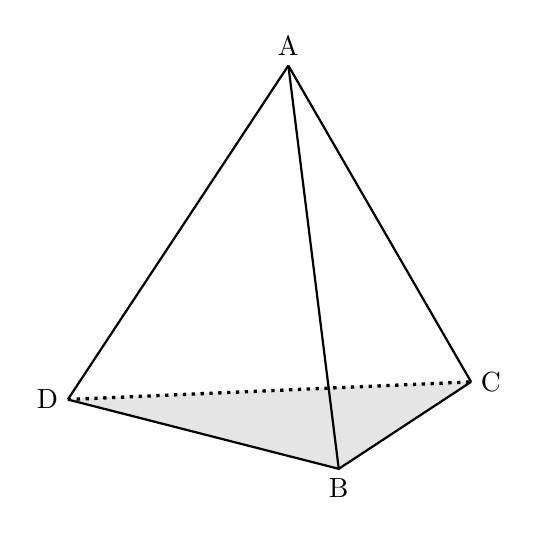
\begin{tikzpicture}[scale=1.6]
        \coordinate (A) at (0.6,0.95);
        \coordinate (B) at (2.75,0.4);
        \coordinate (C) at (3.8,1.09);
        \coordinate (O) at (2.35, 3.6);
        \draw [thick] (O) -- (A);
        \filldraw [gray!20] (A) -- (B) -- (C) -- cycle;
        \draw [thick] (A) -- (B) -- (C);
        \draw [very thick, dotted] (A) -- (C);
        \draw [thick] (O) -- (B);
        \draw [thick] (O) -- (C);
        \node [above]  at (O) {A};
        \node [below]  at (B) {B};
        \node [left]   at (A) {D};
        \node [right]  at (C) {C};
        % \filldraw [red] ($(B)!0.5!(A)$) circle (1pt);
        % \filldraw [red] ($(A)!0.5!(C)$) circle (1pt);
        % \filldraw [red] ($(O)!0.5!(C)$) circle (1pt);
    \end{tikzpicture}
\end{frame}

% \begin{frame}{Solução}
%     \begin{enumerate}
%         \item Escrever \(\vec{AX}\) como uma combinação linear de \(\vec{AD}\), \(\vec{AB}\) e \(\vec{AC}\)
%         \item \label{xpo} Com os pontos do tetraedro pertencentes ao plano, montar 2 vetores LI
%         \item \label{ddo} Com o ponto \(X\) e um dos pontos do tetraedro pertencentes ao plano, montar um vetor e
%             escrevê-lo em uma combinação linear com os 2 vetores encontrados no passo \ref{xpo} igual a zero
%         \item \label{xpl} Escrever o vetor obtido no passo \ref{ddo} como uma combinação linear de \(\vec{AD}\), \(\vec{AB}\) e \(\vec{AC}\)
%         \item \label{ttl} Escrever os vetores obtidos no passo \ref{xpo} como uma combinação linear de \(\vec{AD}\), \(\vec{AB}\) e \(\vec{AC}\)
%         \item Reescrever a combinação linear obtida no passo \ref{ddo} usando os resultados obtidos nos passos \ref{xpl} e \ref{ttl}
%         \item Verificar para qual valor de \(m\) temos uma solução não nula para os coeficientes da combinação linear obtida em \ref{ddo}
%     \end{enumerate}
% \end{frame}



\begin{frame}{Exemplo 3}
    \only<1-2>{
        No tetraedro \(ABCD\), figura anterior, sejam \(M\), \(N\) e \(P\), respectivamente,
        os pontos médios de \(BD\), \(CD\) e \(AC\), e \(G\) o baricentro do triângulo \(MNP\).
        \begin{itemize}
            \item Exprima \(\vec{BG}\) como combinação linear de \(\vec{BA}\), \(\vec{BC}\) e \(\vec{BD}\)
            \item Calcule \(m\) para que o ponto \(X=B+m\vec{BG}\) pertença ao plano da face \(ACD\)
        \end{itemize}
    }
    \only<1-3>{
        \pause
        \textit{Para quem não lembra...}
        \begin{itemize}
            \item O \textit{baricentro} de um triângulo é o ponto onde as retas que contém as medianas se encontram
            \item Uma \textit{mediana} é o segmento que liga um vértice ao ponto médio do lado oposto
            \item Assim, temos que \(G\) é o baricentro do triângulo \(MNP\):

        \end{itemize}
    }
    \only<3>{
        \begin{center}
            \begin{tikzpicture}[scale=2]

                \coordinate (M) at (0,0);
                \coordinate (N) at (2,0);
                \coordinate (P) at (1,{sqrt(3)});
                \draw[thick] (M) -- (N) -- (P) -- cycle;
                \node [left] at (M) {M};
                \node [right] at (N) {N};
                \node [above] at (P) {P};

                \coordinate (Y) at ($(M) !0.5! (P)$);
                \coordinate (X) at ($(P) !0.5! (N)$);
                \coordinate (Z) at ($(M) !0.5! (N)$);

                \node [red,below] at (Z) {Z};
                \node [red,above right] at (X) {X};
                \node [red,above left] at (Y) {Y};

                \draw [thick, red, name path=MX] (M) -- (X);
                \draw [thick, red] (N) -- (Y);
                \draw [thick, red, name path=PZ] (P) -- (Z);

                \path [name intersections={of=MX and PZ,by=G}];
                \node [blue,left] at (G) {G};
            \end{tikzpicture}

        \end{center}
    }
\end{frame}

\begin{frame}{Base}
    \begin{itemize}
        \item Chamamos uma \textit{sequência} de 3 vetores linearmente independente \(E=(\vec{e_1}, \vec{e_2}, \vec{e_3})\)
            de \textbf{base} em \textcolor{blue}{\(R^3\)}
        \item Assim, temos que qualquer vetor \(\vec{u}\) pode ser escrito como
            \[
                \vec{u} = \alpha_1 \vec{e_1} + \alpha_2 \vec{e_2} + \alpha_3 \vec{e_3}
            \]
        \item Cada escalar da \textit{sequência} de escalares \((\alpha_1, \alpha_2, \alpha_3)\) é chamado de
            \textbf{coordenada} do vetor \(\vec{u}\) na base \(E\)
        \item Podemos escrever que \(\vec{u} = (\alpha_1, \alpha_2, \alpha_3)_E\) ou simplesmente
            \(\vec{u} = (\alpha_1, \alpha_2, \alpha_3)\) quando não há dúvidas quanto à base utilizada
    \end{itemize}
\end{frame}

\begin{frame}{Propriedades}
    \begin{itemize}
        \item Se \(\vec{u}=(a_1,a_2,a_3)_E\) e \(\vec{v}=(b_1,b_2,b_3)_E\), então
            \[
                \vec{u}+\vec{v}=(a_1+b_1,a_2+b_2,a_3+b_3)
            \]
        \item Se \(\vec{u}=(a_1,a_2,a_3)_E\), então \(m\vec{u}=(m a_1,m a_2,m a_3)_E\)
        \item Os vetores \(\vec{u}=(a_1,a_2,a_3)_E\) e \(\vec{v}=(b_1,b_2,b_3)_E\) são LD se, e somente se,
            os três determinantes
            \[
                \begin{vmatrix}
                    a_1 & a_2 \\ b_1 & b_2
                \end{vmatrix} \qquad
                \begin{vmatrix}
                    a_1 & a_3 \\ b_1 & b_3
                \end{vmatrix} \qquad
                \begin{vmatrix}
                    a_2 & a_3 \\ b_2 & b_3
                \end{vmatrix}
            \]
            são nulos
        \item Os vetores \(\vec{u}=(a_1,a_2,a_3)_E\), \(\vec{v}=(b_1,b_2,b_3)_E\) e \(\vec{w}=(c_1,c_2,c_3)_E\) são LD se, e somente se,
            \[
                \begin{vmatrix}
                    a_1 & a_2 & a_3 \\ b_1 & b_2 & b_3 \\ c_1 & c_2 & c_3
                \end{vmatrix} = 0
            \]
    \end{itemize}
\end{frame}

\begin{frame}{Módulo e bases ortonormais}
    \begin{itemize}
        \item Os vetores não nulos \(\vec{u}\) e \(\vec{v}\) são \textbf{ortogonais} se existe um representante
            \((A,B)\) de um deles e um representante \((A,C)\) do outro tais que os segmentos AB e AC sejam
            \textit{perpendiculares}
        \item Representa-se por \(\vec{u} \perp \vec{v}\)
        \item O vetor nulo é ortogonal a qualquer vetor
        \item Uma base \((\vec{e_1},\vec{e_2},\vec{e_3})\) é \textbf{ortonormal} se \(\vec{e_1},\vec{e_2},\vec{e_3}\)
            são \textit{unitários} e dois a dois \textit{ortogonais}
        \item Seja \(\vec{u}=(a_1,a_2,a_3)_E\). Se \(E\) é uma base ortonormal, então temos
            que\footnote{Isso só é verdade para bases ortonormais, \textit{tome cuidado}}:
            \[
                ||\vec{u}||=\sqrt{a_1^2+a_2^2+a_3^2}
            \]

    \end{itemize}
\end{frame}

\begin{frame}{Atividade 1}
    Resolva, em sala de aula, os exercícios de 7-2, 7-3, 7-4, 7-5, 7-6, 7-7, 7-8, 7-9, 7-10, 7-11 e 7-12 do livro texto
\end{frame}
